% !TEX root = ../main.tex
%Este trabalho está licenciado sob a Licença Creative Commons Atribuição-CompartilhaIgual 3.0 Não Adaptada. Para ver uma cópia desta licença, visite http://creativecommons.org/licenses/by-sa/3.0/ ou envie uma carta para Creative Commons, PO Box 1866, Mountain View, CA 94042, USA.

\chapter{Representações da série de Fourier e diagramas de espectro}
No capítulo anterior, vimos que uma função periódica pode ser representa como uma série trigonométrica. No entanto, sobretudo em aplicações em Física e Engenharia, a série de Fourier é apresentada em outras formas, a forma harmônica (ou amplitude-fase) e a forma exponencial. Neste capítulo veremos como construir estas representações e introduziremos o conceito de diagramas de espectro de uma função periódica.
\section{Forma harmônica}
A forma harmônica, também chamada de forma amplitude-fase, da série de Fourier de uma função $f(t)$ é dada conforme a seguir:
\begin{equation}
f(t)=A_0+\sum_{n=1}^\infty A_n\cos(w_n t-\theta_n),
\end{equation}
onde $w_n=\frac{2\pi n}{T}$, $A_n$ são constantes não negativas chamadas de amplitude e $\theta_n$ são ângulos de fase. Para relacionar esta representação com a forma trigonométrica, usamos a identidade trigonométrica
\begin{equation}
\cos(a-b)=\cos(a)\cos(b)+\sen(a)\sen(b),
\end{equation}
com $a=w_n t$ e $b=\theta_n$. Assim temos:
\begin{eqnarray*}
f(t)&=&A_0+\sum_{n=1}^\infty A_n\cos(w_n t-\theta_n)\\
&=&A_0+\sum_{n=1}^\infty A_n\left[\cos(w_n t)\cos(\theta_n)+\sen(w_n t)\sen(\theta_n)\right]\\
&=&\underbrace{A_0}_{a_0/2}+\sum_{n=1}^\infty[ \underbrace{A_n\cos(\theta_n)}_{a_n} \cos(w_n t)+\underbrace{A_n\sen(\theta_n)}_{b_n}\sen(w_n t)].
\end{eqnarray*}
Comparando os termos da representação trigonométrica, temos que:
\begin{eqnarray*}
\frac{a_0}{2}&=&A_0\\
a_n&=&A_n\cos(\theta_n)\\
b_n&=&A_n\sen(\theta_n)\\
\end{eqnarray*}
Observe que
\begin{equation}
a_n^2+b_n^2=A_n^2.
\end{equation}
Como $A_n\geq 0$ por hipótese, temos que 
\begin{equation}
A_n=\sqrt{a_n^2+b_n^2}.
\end{equation}
Também temos
\begin{eqnarray*}
\cos(\theta_n)&=&\frac{a_n}{\sqrt{a_n^2+b_n^2}}\\
\sen(\theta_n)&=&\frac{b_n}{\sqrt{a_n^2+b_n^2}}
\end{eqnarray*}
Observe que sempre é possível converter uma forma na outra e os ângulos de fase estão unicamente definidos em cada volta do ciclo trigonométrico.
\begin{ex}Considere um função periódica ($T=4$) dada pelo gráfico
\begin{figure}[!ht]
\begin{center}
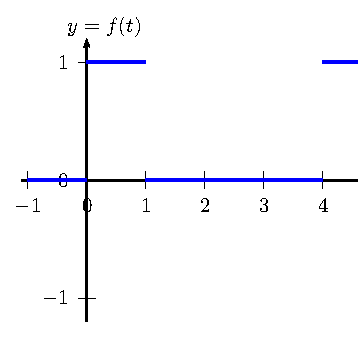
\includegraphics{cap_diagramas_espectro/pics/figura_1}
\end{center}
\end{figure}
Os coeficientes de Fourier são dados por 
\begin{eqnarray*}
\frac{a_0}{2}&=&\frac{1}{4}\int_0^4f(t)dt=\frac{1}{4}\int_0^1 1 dt=\frac{1}{4}\\[10pt]
\end{eqnarray*}
\begin{eqnarray*}
a_n&=&\frac{2}{4}\int_0^4f(t)\cos(w_n t)dt=\frac{1}{2}\int_0^1\cos\left(\frac{\pi n}{2} t\right)dt\\&=&\frac{1}{\pi n}\left[\sen\left(\frac{\pi n}{2} t\right)\right]_0^1\\&=&\left\{\begin{array}{ll} 0,&n\ \hbox{par}\\[8pt]\frac{1}{\pi n}(-1)^{\frac{n-1}{2}}&n\ \hbox{ímpar}  \end{array}\right.
\end{eqnarray*}
\begin{eqnarray*}
b_n&=&\frac{2}{4}\int_0^4f(t)\sen(w_n t)dt=\frac{1}{2}\int_0^1\sen\left(\frac{\pi n}{2} t\right)dt\\&=&\frac{1}{\pi n}\left[-\cos\left(\frac{\pi n}{2} t\right)\right]_0^1\\&=&\left\{\begin{array}{ll} \frac{1}{\pi n},&n\ \hbox{ímpar}\\[8pt] \frac{1}{\pi n}\left(1-(-1)^{\frac{n}{2}}\right)&n\ \hbox{par}  \end{array}\right.\\
\end{eqnarray*}
\begin{table}[ht] 
\begin{center}
   \begin{tabular}{|c|c|c|c|c|}
   \hline
   $n$ & $a_n$ & $b_n$ & $A_n$&$\theta_n  $ \\
   \hline
   &&&&\\
   0& $\frac{1}{2}$ & 0 & $\frac{1}{4}$ & \\
   &&&&\\
   \hline
   &&&&\\
   1&$\frac{1}{\pi}$ & $\frac{1}{\pi}$ & $\frac{\sqrt{2}}{\pi}$ & $\frac{\pi}{4}$ \\
		&&&&\\
		\hline
		 &&&&\\
   2&$0$&$\frac{1}{\pi}$ & $\frac{1}{\pi}$ & $\frac{\pi}{2}$  \\
		&&&&\\
		\hline
		 &&&&\\
   3&$-\frac{1}{3\pi}$&$\frac{1}{3\pi}$& $\frac{\sqrt{2}}{3\pi}$ & $\frac{3\pi}{4}$\\
		&&&&\\
		\hline
		 &&&&\\
   4&$0$&$0$&0&\\
		&&&&\\
		\hline
		&&&&\\
		5&$\frac{1}{5\pi}$&$\frac{1}{5\pi}$&$\frac{\sqrt{2}}{5\pi}$&$\frac{\pi}{4}$ \\
		&&&&\\
		\hline
 \end{tabular}
 \caption{\label{tab_exponential_form}}
   \end{center}
\end{table}
Para escrever a forma harmônica da série de Fourier da função $f(t)$ calculamos as amplitudes $A_n$ e as fases $\theta_n$. Para $n=0$, temos $a_0=\frac{1}{2}$ e, portanto, $A_0=\frac{a_0}{2}=\frac{1}{4}$. Para $n=1$, temos $a_1=b_1=\frac{1}{\pi}$ e, consequentemente, $A_1=\sqrt{\frac{1}{\pi^2}+\frac{1}{\pi^2}}=\frac{\sqrt{2}}{\pi}$ e $\theta_1=\frac{\pi}{4}$. Os cálculos foram repetidos de forma análoga para $n=2,\ 3,\ 4$ e $5$ e apresentados na tabela \ref{tab_exponential_form}. Portanto,
\begin{eqnarray*}
f(t)&=&\frac{1}{4}+\frac{1}{\pi}\left[\sqrt{2}\cos\left(\frac{\pi }{2} t-\frac{\pi}{4}\right)+\cos\left(\pi  t-\frac{\pi}{2}\right)+\right.\\&+&\left.\frac{\sqrt{2}}{3}\cos\left(\frac{3 \pi }{2} t-\frac{3\pi}{4}\right)+\frac{\sqrt{2}}{5}\cos\left(\frac{5 \pi }{2} t-\frac{\pi }{4}\right)+\cdots   \right].
\end{eqnarray*}

\end{ex}
\section{Forma exponencial}
A forma exponencial de uma série de Fourier é obtida quando se substiuem as funções trigonométricas $\sen(w_nt)$ e $\cos(w_nt)$ por suas representações em termos de exponenciais complexos, isto é
\begin{equation}\cos(w_nt)=\frac{e^{iw_nt}+ e^{-iw_nt}}{2}~~~\hbox{e}~~~\sen(w_nt)=\frac{e^{iw_nt}- e^{-iw_nt}}{2i}\end{equation}
\begin{eqnarray*}
f(t)&=&\frac{a_0}{2}+\sum_{n=1}^\infty a_n\cos(w_n t)+\sum_{n=1}^\infty b_n\sen(w_n t)\\
&=&\frac{a_0}{2}+\sum_{n=1}^\infty a_n\left(\frac{e^{iw_nt}+ e^{-iw_nt}}{2}\right)+\sum_{n=1}^\infty b_n\left(\frac{e^{iw_nt}- e^{-iw_nt}}{2i}\right)\\
\end{eqnarray*}
Reagrupando os termos e usando o fato que $\frac{1}{i}=-i$, temos:
\begin{eqnarray}\label{form_exp_1}
f(t)=\frac{a_0}{2}+\sum_{n=1}^\infty \frac{a_n-ib_n}{2}e^{iw_nt}+\sum_{n=1}^\infty \frac{a_n+ib_n}{2}e^{-iw_nt}
\end{eqnarray}
Agora observamos que as definições \ref{coef} dadas por  
\begin{eqnarray*}
   a_0&=& \frac{2}{T}\int_0^T f(t)dt = \frac{2}{T}\int_{-T/2}^{T/2} f(t)dt\\
   a_n&=& \frac{2}{T}\int_0^T f(t)\cos(w_n t)dt = \frac{2}{T}\int_{-T/2}^{T/2} f(t)\cos(w_nt)dt\\
   b_n&=& \frac{2}{T}\int_0^T f(t)\sen(w_n t)dt = \frac{2}{T}\int_{-T/2}^{T/2} f(t)\sen(w_nt)dt
  \end{eqnarray*}
Embora estas expressões estejam definadas apenas para $n>0$, elas fazem sentidos para qualquer $n$ inteiro. Neste caso, valem as seguintes identidades:
\begin{equation}a_{-n}=a_n,~~b_{-n}=-b_{n}~~b_0=0.\end{equation}
onde se usou que $w_{-n}=\frac{2\pi (-n)}{T}=-\frac{2\pi n}{T}=-w_n$ e a paridade das funções cosseno e seno.
Estendendo estas definições para qualquer inteiro, introduzimos os coeficientes $C_n$ dados por:
\begin{equation}\label{def_cn}
C_n = \frac{a_n - ib_n}{2}
\end{equation}
Observe que estes coeficientes estão definidos para para número inteiro $n$, assim temos:
\begin{equation}
C_0 = \frac{a_0 - ib_0}{2}=\frac{a_0}{2}
\end{equation}
e
\begin{equation}
C_{-n} = \frac{a_{-n} - ib_{-n}}{2}=\frac{a_{n} + ib_{n}}{2}
\end{equation}
Substituindo estas expressões para $C_0$, $C_{n}$ e $C_{-n}$ em (\ref{form_exp_1}), obtemos:
\begin{eqnarray*}
f(t)=C_0+\sum_{n=1}^\infty C_n e^{iw_nt}+\sum_{n=1}^\infty C_{-n}e^{-iw_nt}
\end{eqnarray*}
Escrevemos agora esta última expressão em um único somatório:
\begin{eqnarray}\label{forma_exp}
f(t)=\sum_{n=-\infty}^\infty C_n e^{iw_nt}
\end{eqnarray}
onde se usou que $w_{-n}=\frac{2\pi (-n)}{T}=-\frac{2\pi n}{T}=-w_n$
Observamos também que os coeficientes $C_n$ podem ser escritos das seguinte forma mais enxuta:
\begin{eqnarray*}
C_n &=& \frac{a_n - ib_n}{2}\\
&=& \frac{1}{T}\int_0^Tf(t)\left[\cos(w_n t)-i\sen(w_n t)\right]dt\\
&=&\frac{1}{T}\int_0^Tf(t)e^{-iw_nt}dt =\frac{1}{T}\int_{-T/2}^{T/2}f(t)e^{-iw_nt}dt 
\end{eqnarray*}
\begin{ex}{\label{ex_exp_1}} A função $f(t)$ dada no exemplo \ref{ex_triangular} pode ser escrita na forma exponencial com os seguintes coeficientes:
\begin{equation}C_0=\frac{a_0}{2}=\frac{1}{2}\end{equation}
\begin{equation}C_n=\frac{a_n-ib_n}{2}=\frac{2\frac{(-1)^n-1}{\pi^2n^2}+0}{2}=\frac{(-1)^n-1}{\pi^2n^2},~~n\neq 0\end{equation}
\end{ex}
\begin{ex}{\label{ex_exp_2}} A função $g(t)$,
\begin{equation}
g(t)=\frac{4}{\pi}\left(\sen(\pi t)+\frac{1}{3}\sen(3\pi t)+\frac{1}{5}\sen(5\pi t)+\cdots\right),
\end{equation}
calculada no exemplo \ref{ex_quadrada} pode ser escrita na forma exponencial com os seguintes coeficientes:
\begin{equation}C_0=\frac{a_0}{2}=0\end{equation}
e
\begin{equation}C_n=\frac{a_n-ib_n}{2}=\frac{0-i2\frac{1-(-1)^n}{\pi n}}{2}=i\frac{(-1)^n-1}{\pi n},~~n\neq 0.\end{equation}
Logo,
\begin{equation}
g(t)=\cdots+\frac{2i}{5\pi}e^{-5i\pi t}+\frac{2i}{3\pi}e^{-3i\pi t}+\frac{2i}{\pi}e^{-i\pi t}-\frac{2i}{\pi}e^{i\pi t}-\frac{2i}{3\pi}e^{3i\pi t}-\frac{2i}{5\pi}e^{5i\pi t}-\cdots,
\end{equation}
\end{ex}

\subsection*{Exercícios resolvidos}
\begin{exeresol}

  Considere a função $f(t)=8\cos^4(t)$. 

\begin{itemize}
 \item[a)] Obtenha a frequência fundamental.
 \item[b)] Obtenha o período fundamental.
 \item[c)] Construa forma trigonométrica da série de Fourier de $f(t)$.
 \item[d)] Construa a forma exponencial da série de Fourier de $f(t)$.
 \item[e)] Esboce os diagramas de espectro.
\end{itemize}
\begin{resol}
Usando o binômio de Newton, obtemos a seguinte identidade trigonométrica:
\begin{eqnarray*}
8\cos^4(t)&=&8\left(\frac{e^{it}+e^{-it}}{2}\right)^4\\
&=&\frac{e^{4it}+ 4 e^{3it}e^{-it}+ 6 e^{2it}e^{-2it}+ 4 e^{it}e^{-3it} +e^{-4it} }{2} \\
&=&\frac{1}{2}e^{-4it}+2 e^{-2it}+3  + 2 e^{2it} +\frac{1}{2}e^{4it} \quad \hbox{(forma exponencial)}\\
&=&3+\frac{e^{4it}+e^{-4it} }{2}+4\frac{  e^{2it}+  e^{-2it} }{2}\\
&=&3+4\cos(2t)+\cos(4t)\quad \hbox{(forma trigonométrica)}\\
\end{eqnarray*}

Observe que a frequência fundamental é $w=2$ e o período fundamental é $\pi$. O diagrama de espectro de fase é zero em todas as frequências e o diagrama de espectro de amplitudes é dado no gráfico abaixo:

\begin{center}
  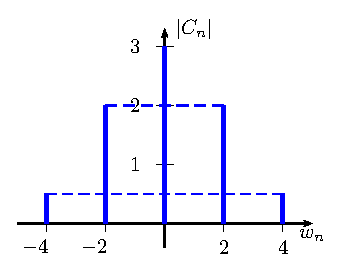
\includegraphics{cap_diagramas_espectro/pics/diagrama_3}
\end{center}
\end{resol}


\end{exeresol}

\subsection*{Exercícios}
\begin{exer} Mostre que se $f(t)=\sum_{n=-\infty}^\infty C_n e^{i w_n t}$ é uma função real, então $C_{-n}=\overline{C_n}$. Em especial, $|C_{-n}|=|C_n|$.
\end{exer}

\section{Diagramas de espectro}
Diagramas espectro são representações gráficas dos coeficientes de Fourier $C_n$ associados a uma função periódica $f(t)$. Como os coeficientes $C_n$ são números complexos, é comum representá-los na forma de módulo e fase, isto é:
\begin{equation}C_n = |C_n|e^{i\phi_n}.\end{equation}
O ângulo de fase assim definido coincide com o conceito de argumento do número $C_n$.
\begin{ex} A função 
\begin{equation}f(t)=-1+2\cos(t)+4\sen(2t)\end{equation}
é periódica com periodo fundamental $2\pi$ e pode ser escrita na forma exponencial da seguinte forma:
\begin{eqnarray*}
f(t)&=&-1+2\left(\frac{e^{it}+e^{-it}}{2}\right)+4\left(\frac{e^{2it}-e^{-2it}}{2i}\right)\\
&=&2i e^{-2it} + e^{-it}-1+e^{it}- 2ie^{2it}
\end{eqnarray*}
Assim, identificamos cinco coeficientes não nulos:
\begin{equation*}
\begin{array}{lclcll}
 C_{-2}&=&2i=2e^{\frac{i\pi}{2}} &\Longrightarrow& |C_{-2}|=2, ~~ &\phi_{-2}=\frac{\pi}{2}\\
 C_{-1}&=&1 &\Longrightarrow& |C_{-1}|=1, ~~ &\phi_{-1}=0\\
 C_{0}&=&-1=1e^{\pi} &\Longrightarrow& |C_{0}|=1, ~~ &\phi_0=\pi\\
 C_{1}&=&1 &\Longrightarrow& |C_{1}|=1, ~~ &\phi_1=0\\
 C_{2}&=&-2i=2e^{\frac{-i\pi}{2}} &\Longrightarrow& |C_{2}|=2, ~~ &\phi_2=-\frac{\pi}{2}
\end{array}
 \end{equation*}
Os digramas de espectro de amplitude e fase são dados a seguir:
\begin{figure}[!ht]
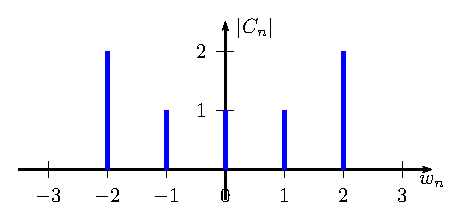
\includegraphics{cap_diagramas_espectro/pics/figura_2}
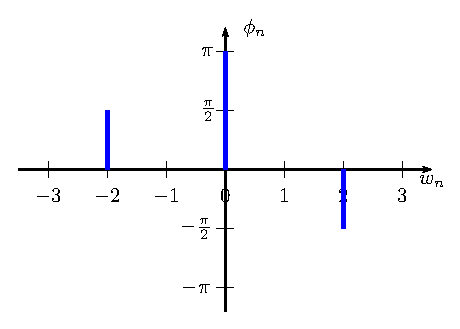
\includegraphics{cap_diagramas_espectro/pics/figura_3}
\end{figure}
\end{ex}
\begin{ex} As primeiras raias do digrama de espectro da função do exemplo \ref{ex_exp_2},
\begin{equation}
g(t)=\cdots+\frac{2i}{5\pi}e^{-5i\pi t}+\frac{2i}{3\pi}e^{-3i\pi t}+\frac{2i}{\pi}e^{-i\pi t}-\frac{2i}{\pi}e^{i\pi t}-\frac{2i}{3\pi}e^{3i\pi t}-\frac{2i}{5\pi}e^{5i\pi t}-\cdots,
\end{equation}
são dados na figura a seguir
\begin{figure}[!ht] 
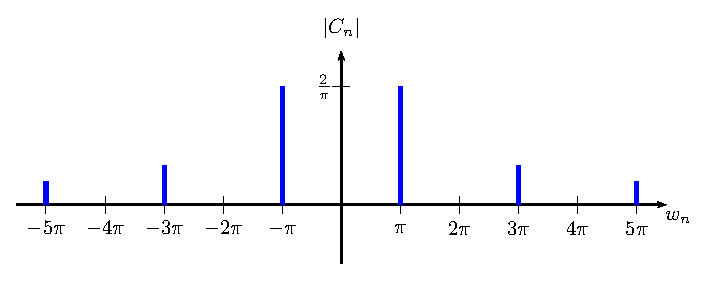
\includegraphics{cap_diagramas_espectro/pics/figura_4}
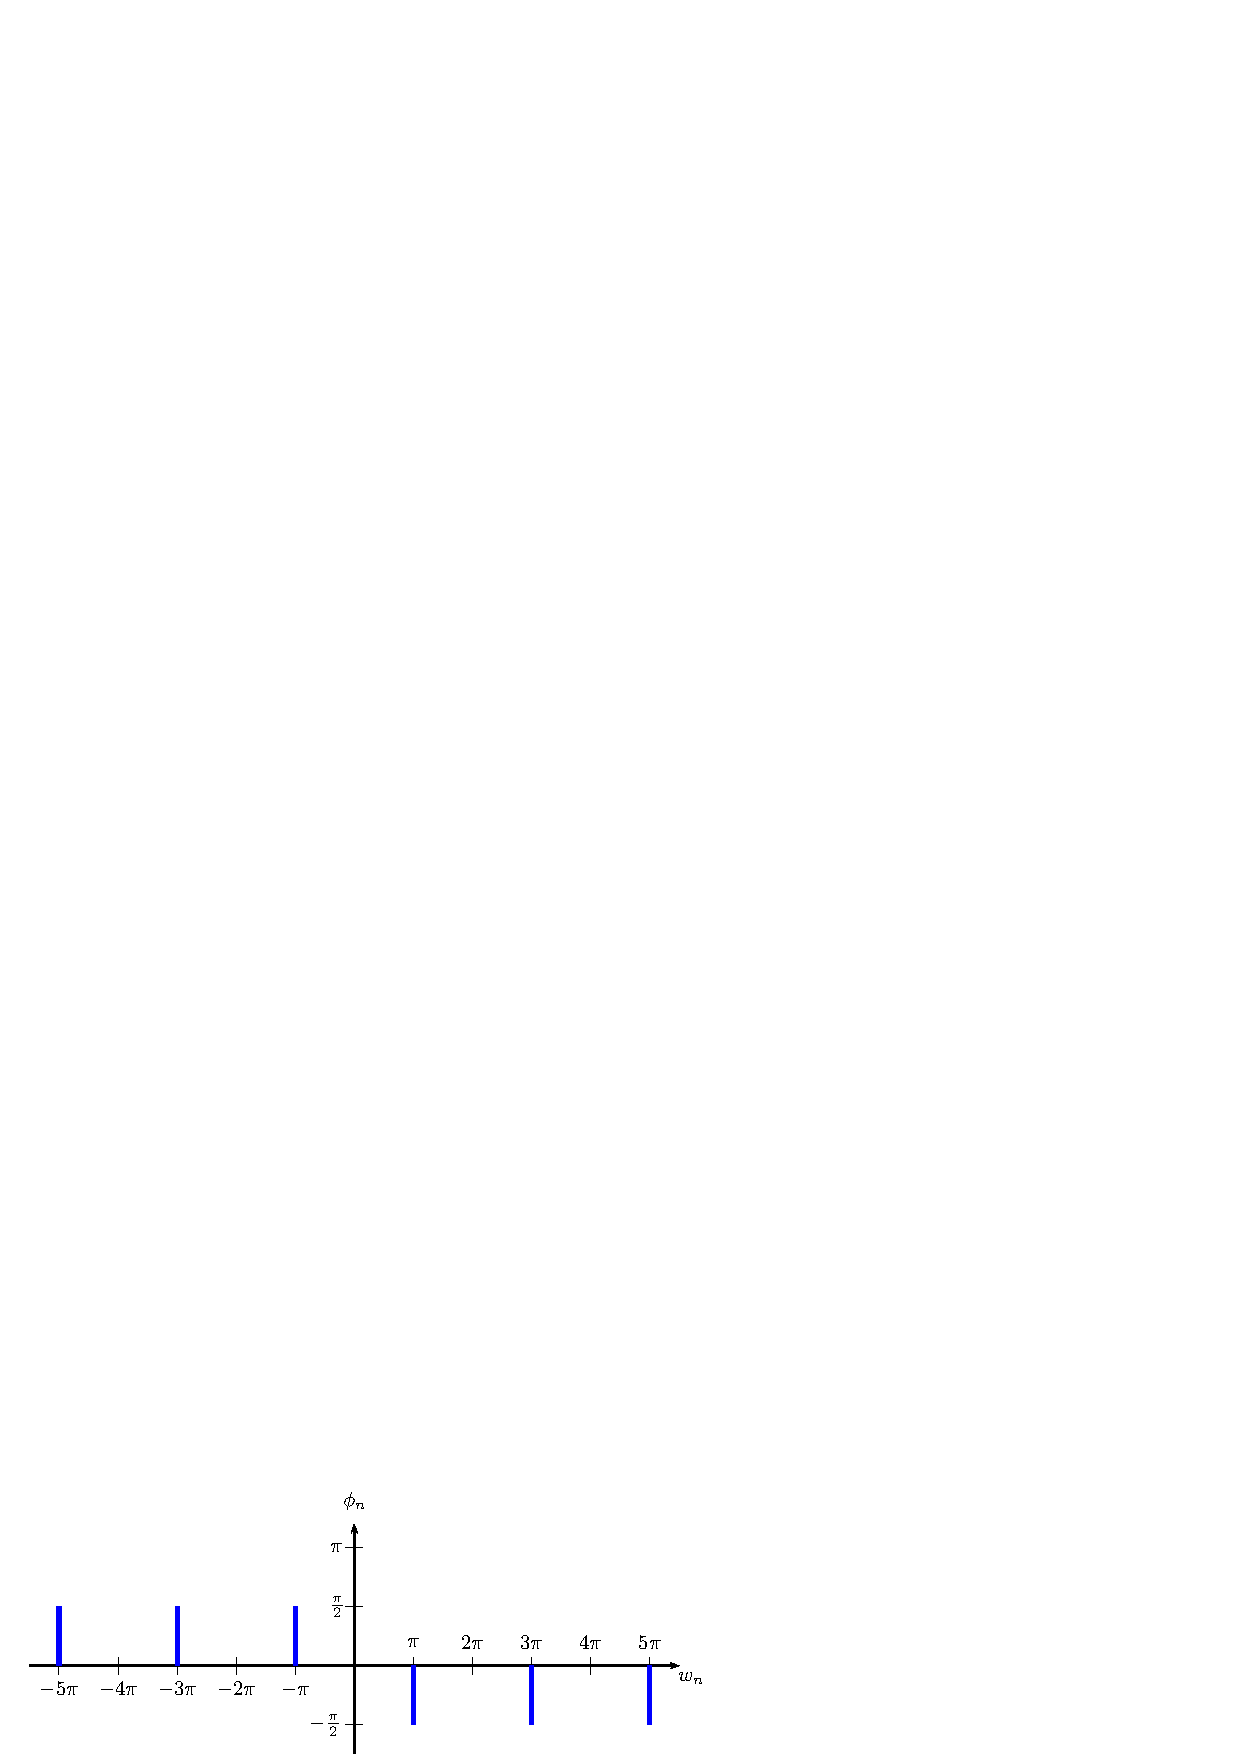
\includegraphics{cap_diagramas_espectro/pics/figura_5}
\end{figure}
\end{ex}
\subsection*{Exercícios}
\begin{exer}
Esboce os diagramas de amplitude e fase do espectro das seguintes funções periódicas:
\begin{itemize}
\item[a)] $f(t)=\sen(t)$\
\item[b)] $f(t)=3\cos(\pi t)$
\item[c)] $f(t)=1+4\cos(\pi t)$
\item[d)] $f(t)=2\cos^2(2\pi t)$
\item[e)] $f(t)=8\sen^3(2\pi t)+2\cos(6\pi t)$
\item[f)] $f(t)=\sen(2\pi t)+\cos(3\pi t)$
\end{itemize}
Observação: Considere a fase $\phi$ no intervalo $-\pi< \phi\leq \pi$
\end{exer}
\begin{resp}
 \begin{itemize}
  \item [a)]
 Observe que: 
 \begin{equation}
  \sen(t)=\frac{1}{2i}\left(e^{it}-e^{-it}\right)= \frac{i}{2}e^{-it} - \frac{i}{2}e^{it}
\end{equation} 
e a frequência angular fundamental é $w_F=1$. Veja os diagramas de espectro na figura abaixo.

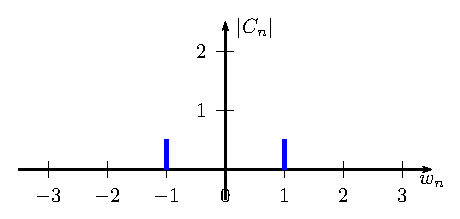
\includegraphics{cap_diagramas_espectro/pics/figura_6}~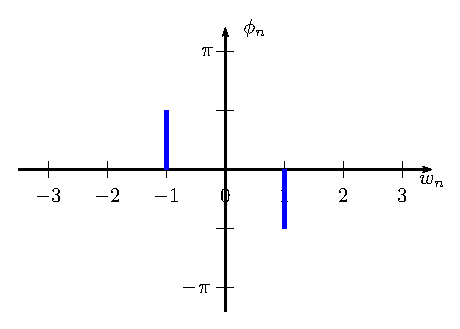
\includegraphics{cap_diagramas_espectro/pics/figura_7}


\item [b)]
 Observe que:
 \begin{equation}3\cos(\pi t)=\frac{3}{2}\left(e^{i\pi t}+e^{-i\pi t}\right)= \frac{3}{2}e^{-i\pi t} + \frac{3}{2}e^{i\pi t}
\end{equation} 
 e a frequência angular fundamental é $w_F=\pi$. Veja os diagramas de espectro na figura abaixo. 

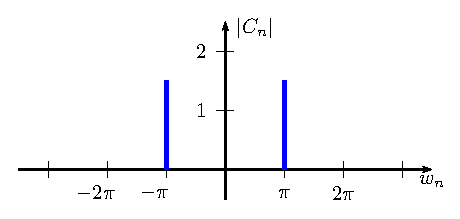
\includegraphics{cap_diagramas_espectro/pics/figura_8}~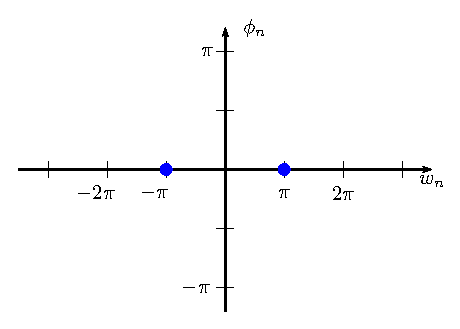
\includegraphics{cap_diagramas_espectro/pics/figura_9}

\item [c)]
Observe que:
 \begin{equation}
  1+4\cos(\pi t)=1+2\left(e^{i\pi t}+e^{-i\pi t}\right)= 1+2e^{-i\pi t} + 2e^{i\pi t}\end{equation}
  
  e a frequência angular fundamental é $w_F=\pi$.  Veja os diagramas de espectro na figura abaixo. 

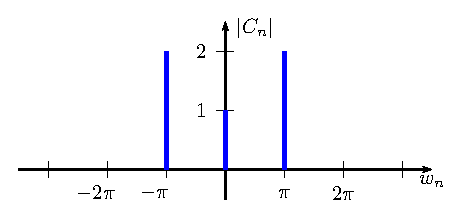
\includegraphics{cap_diagramas_espectro/pics/figura_10}~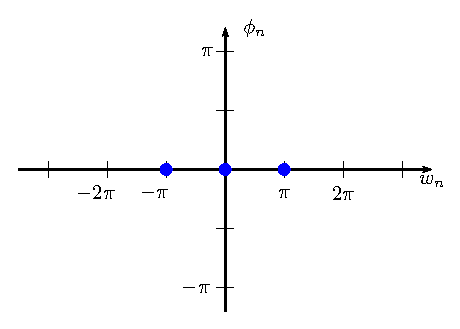
\includegraphics{cap_diagramas_espectro/pics/figura_11}

\item [d)]
 Observe que:
 \begin{equation}
  2\cos^2(2\pi t)=2\left(\frac{e^{2i\pi t}+e^{-2i\pi t}}{2}\right)^2= \frac{e^{-4i\pi t} +2+ e^{4i\pi t}}{2}= \frac{1}{2}e^{-4i\pi t} +1+ \frac{1}{2}e^{4i\pi t}\end{equation} 
  e a frequência angular fundamental é $w_F=4\pi$.  Veja os diagramas de espectro na figura abaixo. 

  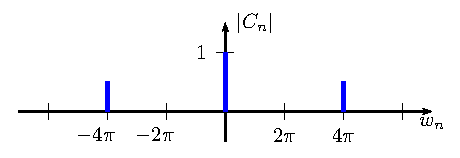
\includegraphics{cap_diagramas_espectro/pics/figura_12}~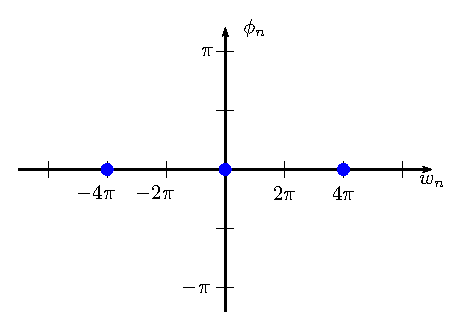
\includegraphics{cap_diagramas_espectro/pics/figura_13}

\item [e)]
 Observe que 
\begin{eqnarray*}
8\sen^3(2\pi t)+2\cos(6\pi t)&=&8\left(\frac{e^{2i\pi t}-e^{-2i\pi t}}{2i}\right)^3+2\left(\frac{e^{6i\pi t}+e^{-6i\pi t}}{2}\right)\\&=& (i+1)e^{6i\pi t}-3 i e^{2i\pi t}+3 i e^{-2i\pi t}+(1-i)e^{-6i\pi t}\\&=&\sqrt{2}e^{\frac{\pi}{4}i} e^{6i\pi t}+3e^{-\frac{\pi}{2}i} e^{2i\pi t}+3 e^{\frac{\pi}{2}i} e^{-2i\pi t}+\sqrt{2}e^{-\frac{\pi}{4}i}e^{-6i\pi t} 
\end{eqnarray*}
e a frequência angular fundamental é $w_F=2\pi$.  Veja os diagramas de espectro na figura abaixo.

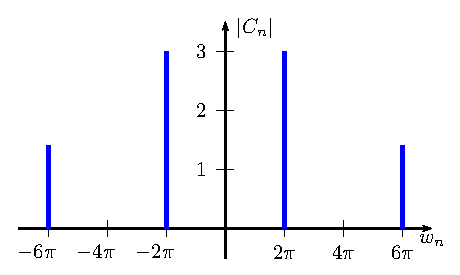
\includegraphics{cap_diagramas_espectro/pics/figura_14}~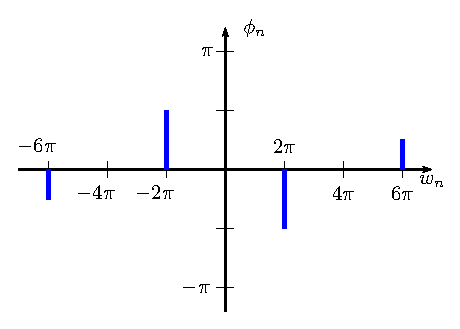
\includegraphics{cap_diagramas_espectro/pics/figura_15}

\item [f)]
 Observe que 
\begin{eqnarray*}
\sen(2\pi t)+\cos(3\pi t)&=&\left(\frac{e^{2i\pi t}-e^{-2i\pi t}}{2i}\right)+\left(\frac{e^{3i\pi t}+e^{-3i\pi t}}{2}\right)\\
&=& -\frac{i}{2}e^{2i\pi t}+\frac{i}{2}e^{-2i\pi t}+\frac{1}{2}e^{3i\pi t}+\frac{1}{2}e^{-3i\pi t}
\end{eqnarray*}
e a frequência angular fundamental é $w_F=\pi$ (ver exercício \ref{freq_fund} na página \pageref{freq_fund}).  Veja os diagramas de espectro na figura abaixo.
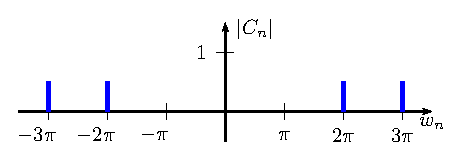
\includegraphics{cap_diagramas_espectro/pics/figura_16}
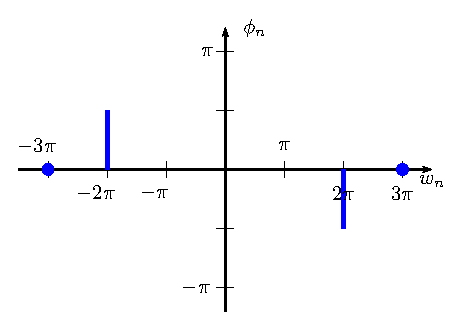
\includegraphics{cap_diagramas_espectro/pics/figura_17}
\end{itemize}
\end{resp}
\begin{exer}
Esboce os diagramas de amplitude e fase do espectro, indicando pelo menos as cinco primeiras raias positivas e negativas, das seguintes funções periódicas:
\begin{itemize}
\item[a)] $f(t)=\sum_{n=-\infty}^\infty \frac{e^{i \pi n t}}{n^2+1}$
\item[b)] $f(t)=\sum_{n=1}^\infty \frac{\sen(nt)}{n^2}$
\end{itemize}
\end{exer}
\begin{resp} 
\begin{itemize}
\item [a)] Observe que $f(t)$ já está na forma exponencial e a frequência fundamental é $w_F=\pi$. Também temos:
\begin{equation}
\begin{array}{|c|c|c|c|}
\hline
n&\omega_n&|C_n|&\phi_n\\
\hline
-5&-5\pi &\frac{1}{(-5)^2+1}=\frac{1}{26}&0\\
\hline
-4&-4\pi &\frac{1}{(-4)^2+1}=\frac{1}{17}&0\\
\hline
-3&-3\pi &\frac{1}{(-3)^2+1}=\frac{1}{10}&0\\
\hline
-2&-2\pi &\frac{1}{(-2)^2+1}=\frac{1}{5}&0\\
\hline
-1&-\pi &\frac{1}{(-1)^2+1}=\frac{1}{2}&0\\
\hline
0&0 &\frac{1}{(0)^2+1}=1&0\\
\hline
1&1\pi &\frac{1}{1^2+1}=\frac{1}{2}&0\\
\hline
2&2\pi &\frac{1}{2^2+1}=\frac{1}{5}&0\\
\hline
3&3\pi &\frac{1}{3^2+1}=\frac{1}{10}&0\\
\hline
4&4\pi &\frac{1}{4^2+1}=\frac{1}{17}&0\\
\hline
5&5\pi &\frac{1}{5^2+1}=\frac{1}{26}&0\\
\hline
\end{array}
\end{equation}
Veja o diagrama de amplitude na figura abaixo.

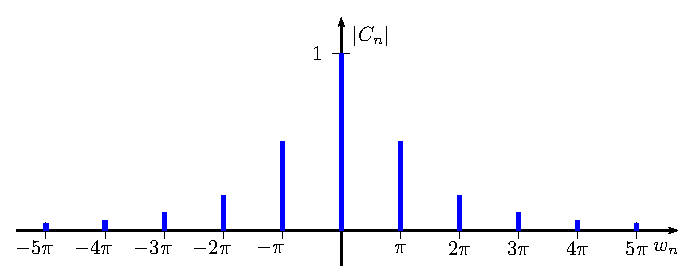
\includegraphics{cap_diagramas_espectro/pics/figura_18}
\item [b)]
 Começamos escrevendo a função $f(t)=\sum_{n=1}^\infty \frac{\sen(nt)}{n^2}$ na forma exponencial:
\begin{eqnarray*}
\sum_{n=1}^\infty \frac{\sen(nt)}{n^2}&=&\sum_{n=1}^\infty \frac{1}{n^2}\left(\frac{e^{int}-e^{-int}}{2i}\right)\\
&=&\sum_{n=1}^\infty \frac{1}{2i n^2} e^{int}+\sum_{n=1}^\infty\left( -\frac{1}{2i n^2}e^{-int}\right)\\
&=&\sum_{n=1}^\infty \left(-\frac{i}{2 n^2} e^{int}\right)+\sum_{n=-1}^{-\infty}\frac{i}{2 n^2}e^{int}.
\end{eqnarray*}
A frequência angular fundamental é $w_F=1$ e as amplitudes e fases são dados na tabela abaixo.
\begin{equation}
\begin{array}{|c|c|c|}
\hline
\omega_n=n&|C_n|&\phi_n\\
\hline
-5&\frac{1}{50}&\frac{\pi}{2}\\
\hline
-4 &\frac{1}{32}&\frac{\pi}{2}\\
\hline
-3 &\frac{1}{18}&\frac{\pi}{2}\\
\hline
-2 &\frac{1}{8}&\frac{\pi}{2}\\
\hline
-1 &\frac{1}{2}&\frac{\pi}{2}\\
\hline
0 &0&-\\
\hline
1 &\frac{1}{2}&-\frac{\pi}{2}\\
\hline
2 &\frac{1}{8}&-\frac{\pi}{2}\\
\hline
3 &\frac{1}{18}&-\frac{\pi}{2}\\
\hline
4 &\frac{1}{32}&-\frac{\pi}{2}\\
\hline
5 &\frac{1}{50}&-\frac{\pi}{2}\\
\hline
\end{array}
\end{equation}
Veja os diagramas de espectro na figura abaixo.

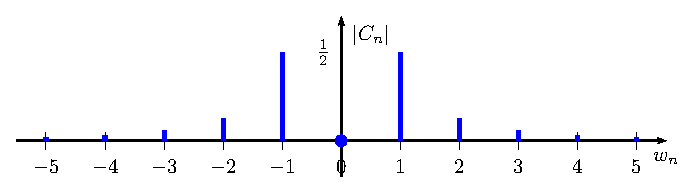
\includegraphics{cap_diagramas_espectro/pics/figura_19}

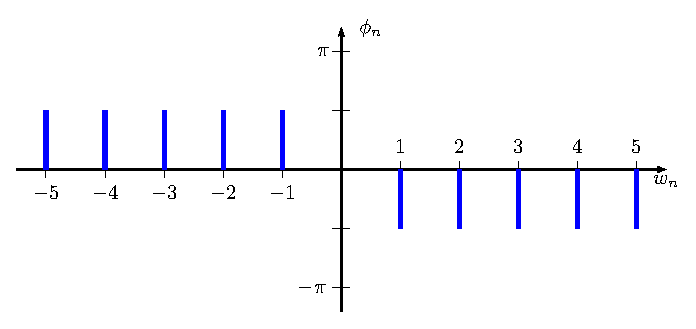
\includegraphics{cap_diagramas_espectro/pics/figura_20}

\end{itemize}
\end{resp}
\begin{exer}Esboce os diagramas de espectro das séries de Fourier dos problemas \ref{Fourier_8} e \ref{Fourier_9} da página \pageref{Fourier_8}.
\end{exer}
\begin{resp}
\begin{itemize}
\item[a)] Problema \ref{Fourier_8} item a:
\begin{eqnarray*}
f(t)&=&\frac{2}{\pi}- \frac{4}{\pi}\sum_{n=1}^\infty \frac{\cos(2n\pi t)}{4n^2-1}\\
&=&\frac{2}{\pi}- \frac{4}{\pi}\sum_{n=1}^\infty \frac{1}{4n^2-1}\left(\frac{e^{2 n\pi it}+e^{-2n\pi it}}{2}\right)\\
&=&\frac{2}{\pi}- \sum_{n=1}^\infty \frac{2}{\pi(4n^2-1)}e^{2 n\pi it}- \sum_{n=-1}^{-\infty} \frac{2}{\pi(4n^2-1)}e^{2n\pi it}
  \end{eqnarray*}
Veja os diagramas de espectro na figura abaixo.

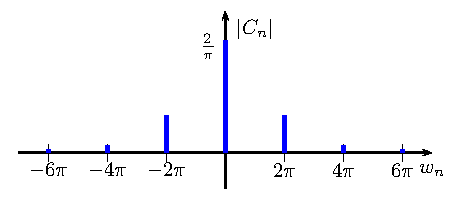
\includegraphics{cap_diagramas_espectro/pics/figura_21}~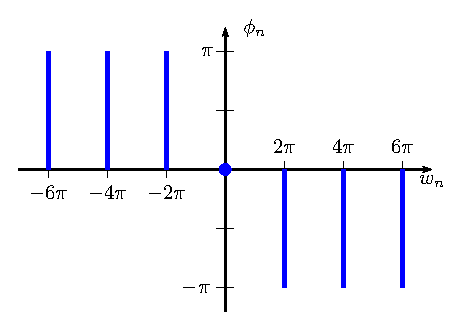
\includegraphics{cap_diagramas_espectro/pics/figura_22}

\item[b)] Problema \ref{Fourier_9} item
\begin{eqnarray*}
h(t)&=&\frac{2}{\pi}- \frac{4}{\pi}\sum_{n=1}^\infty (-1)^n\frac{\cos(2n\pi t)}{4n^2-1}\\
&=&\frac{2}{\pi}- \frac{4}{\pi}\sum_{n=1}^\infty \frac{(-1)^n}{4n^2-1}\left(\frac{e^{2 n\pi it}+e^{-2n\pi it}}{2}\right)\\
&=&\frac{2}{\pi}- \sum_{n=1}^\infty \frac{2(-1)^n}{\pi(4n^2-1)}e^{2 n\pi it}- \sum_{n=-1}^{-\infty} \frac{2(-1)^n}{\pi(4n^2-1)}e^{2n\pi it}
  \end{eqnarray*}
	Veja os diagramas de espectro na figura abaixo.

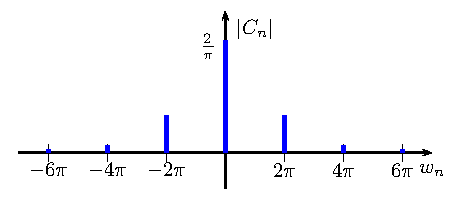
\includegraphics{cap_diagramas_espectro/pics/figura_23}~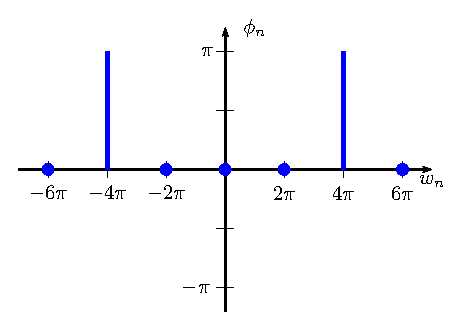
\includegraphics{cap_diagramas_espectro/pics/figura_24}

\end{itemize}
\end{resp}

\begin{exer} Mostre que se $f(t)$ é um deslocamento no tempo de $g(t)$, isto é, $f(t)=g(t-k)$, então os coeficiente de Fourier $C_n^f$ da função $f$ e $C_n^g$ da função $g$ são iguais em módulo e, portanto, possuem o mesmo diagrama de espectro de amplitude.
\end{exer}
